\documentclass[12pt,oneside]{book}
\newcommand{\TITLE}{Mécanique}
\usepackage[utf8]{inputenc}
\usepackage[margin=0.5in]{geometry}
\usepackage[usestackEOL]{stackengine}
\usepackage{amsmath , esint,braket,lmodern,mhchem,bohr,lewis,chemfig,draftwatermark,xcolor,graphicx , amssymb ,ragged2e , listings , siunitx , float , eqparbox, centernot , esvect , bm , fancyhdr , fourier-orns}
\usepackage[ddmmyyyy]{datetime}
\usepackage{fourier-orns}
\usepackage{changepage}
\usepackage{bbm}\usepackage{chngcntr}
\usepackage{hyperref}
\usepackage{ifthen}
\usepackage[many]{tcolorbox}
\DeclareMathOperator{\sech}{sech}
\DeclareMathOperator{\csch}{csch}
\DeclareMathOperator{\arcsec}{arcsec}
\DeclareMathOperator{\arccot}{arcCot}
\DeclareMathOperator{\arccsc}{arcCsc}
\DeclareMathOperator{\arccosh}{arcCosh}
\DeclareMathOperator{\arcsinh}{arcsinh}
\DeclareMathOperator{\arctanh}{arctanh}
\DeclareMathOperator{\arcsech}{arcsech}
\DeclareMathOperator{\arccsch}{arcCsch}
\DeclareMathOperator{\arccoth}{arcCoth} 
\DeclareMathOperator{\grad}{\vv{\text{grad}}} 
\DeclareMathOperator{\conj}{^*} 
\DeclareMathOperator{\vect}{vv} 
\DeclareMathOperator{\Vect}{\text{Vect}} 
\DeclareMathOperator{\degree}{c^\circ} 
\DeclareMathOperator{\degre}{^\circ} 
\DeclareMathOperator{\transpose}{^\dagger} 
\DeclareMathOperator{\adjoint}{^\dagger} 

\newcommand{\moyenne}[1]{\langle #1 \rangle} 
\newcommand{\lagrange}{\mathcal{L}}
\newcommand{\fourier}{\mathcal{F}}
\newcommand{\hilbert}{\mathcal{H}}
\newcommand{\p}{\mathcal{P}}
\newcommand{\x}{\chi}
\newcommand{\ve}[1]{\vv{#1}}
\newcommand{\push}[1]{\begin{adjustwidth}{5mm}{}#1\end{adjustwidth}}
\newcommand{\operator}[1]{\widehat{#1}}
\newcommand{\HRule}{\rule{\linewidth}{0.5mm}} % Defines a new command for the horizontal lines, change thickness here
\renewcommand{\chaptermark}[1]{\markboth{\MakeUppercase{#1}}{}}
\renewcommand{\headrule}{%
\vspace{-8pt}\hrulefill
\raisebox{-2.1pt}{\quad\decofourleft\decotwo\decofourright\quad}\hrulefill}
\definecolor{myred}{RGB}{255, 14, 0}
\everymath{\displaystyle}

\def\changemargin#1{\list{}{\leftmargin#1}\item[]}
\let\endchangemargin=\endlist 

\makeatletter
\newcommand*{\rom}[1]{\expandafter\@slowromancap\romannumeral #1@}%roman numbers
\makeatother

%hyperlink shit

\hypersetup{
    colorlinks,
    citecolor=black,
    filecolor=black,
    linkcolor=black,
    urlcolor=black
}
% Table specail cell , it's for making line break in table cell
\newcommand{\specialcell}[2][c]{%
  \begin{tabular}[#1]{@{}c@{}}#2\end{tabular}}

  \definecolor{main}{HTML}{5989cf}    % setting main color to be used
\definecolor{sub}{HTML}{cde4ff}     % setting sub color to be used

\tcbset{
    sharp corners,
    colback = white,
    before skip = 0.2cm,    % add extra space before the box
    after skip = 0.5cm      % add extra space after the box
}   
\newtcolorbox{boxH}{
    colback = sub, 
    colframe = main, 
    boxrule = 0pt, 
    leftrule = 6pt % left rule weight
}
\newtcolorbox{gpt}{
    sharpish corners, % better drop shadow
    boxrule = 0pt,
    toprule = 4.5pt, % top rule weight
    enhanced,
    fuzzy shadow = {0pt}{-2pt}{-0.5pt}{0.5pt}{black!35} % {xshift}{yshift}{offset}{step}{options} 
}
\definecolor{codegreen}{rgb}{0,0.6,0}
\definecolor{codegray}{rgb}{0.5,0.5,0.5}
\definecolor{codepurple}{rgb}{0.58,0,0.82}
\definecolor{backcolour}{rgb}{0.95,0.95,0.92}

\lstdefinestyle{mystyle}{
    backgroundcolor=\color{backcolour},   
    commentstyle=\color{codegreen},
    keywordstyle=\color{magenta},
    numberstyle=\tiny\color{codegray},
    stringstyle=\color{codepurple},
    basicstyle=\ttfamily\footnotesize,
    breakatwhitespace=false,         
    breaklines=true,                 
    captionpos=b,                    
    keepspaces=true,                 
    numbers=left,                    
    numbersep=5pt,                  
    showspaces=false,                
    showstringspaces=false,
    showtabs=false,                  
    tabsize=2,
    basicstyle = \small
}

\lstset{style=mystyle}
\SetWatermarkAngle{45} 
\SetWatermarkLightness{.99} 
\SetWatermarkFontSize{0.1cm} 
\SetWatermarkScale{0} 
\SetWatermarkText{supahaka}


\begin{document}
\pagestyle{fancy}
\fancyhf{}
\fancyfoot[R]{Tenji$_\text{org}$}
\fancyfoot[C]{\thepage}
\fancyfoot[L]{\tiny www.tenji.org}
\fancyhead[RO]{\nouppercase{\leftmark\hfill\TITLE}}


\DraftwatermarkOptions{stamp=false}
    \begin{titlepage}
        \begin{center}
            \vspace*{5cm}
            \Huge
            \HRule \\[0.4cm]
            \textbf{Project Tenji: \\ \TITLE}\\
            \Large 
            \HRule \\[1.5cm]
            \vspace{2cm}
            \vfill
        \end{center}
        \vfill
        { \scriptsize Project Tenji \copyright 2024 by Khalil Salahat and Mohamad El Moussawi  \\}
        { \scriptsize Hosted at tenji.org , contact : contact@tenji.org \\}
        { \scriptsize \NOTICEE  \\}
    \end{titlepage} 
    \tableofcontents
\DraftwatermarkOptions{stamp=true}
\part{Mécanique General}
\chapter{Mécanique newtonienne}
\section{Énoncés des lois de Newton}
\begin{itemize}
    \item Loi d'inertie \\
    Une particule isolée, sur laquelle n'agit aucune force extérieure, reste au repos ou conserve un mouvement rectiligne uniforme.
    \begin{center}
        \boxed{\vv{F} = \vv{0} \Longleftrightarrow \vv{v} = \vv{cte}}
    \end{center}
    \item Loi fondamentale de la dynamique
    \begin{itemize}
        \item $\vv{F} = m\vv{a}$
        \begin{itemize}
            \item $\vv{a} = \frac{d\vv{v}}{dt}$
            \item $\vv{v} = \frac{d\vv{r}}{dt}$
            \item $\vv{r} = \vv{OM}$ ($O$ est l'origine, $M$ est le point où $\vv{F}$ agit)
        \end{itemize}
        \item $\vv{F} = \frac{d\vv{P}}{dt}$ (avec $\vv{P} = m\vv{v}$ quantité de mouvement)
    \end{itemize}
    \item Principe de l'action et de la réaction : $\vv{F_{12}} = -\vv{F_{21}}$
\end{itemize}
\pagebreak
\section{Loi de conservation pour un point matériel}
\begin{itemize}
    \item Conservation de la quantité de mouvement \\
    Si $\vv{F} = 0$, alors $\vv{F} = \frac{d\vv{P}}{dt} = \vv{0} \implies \vv{P} = \vv{cte}$
    \item Conservation du moment angulaire
    \begin{center}
        \begin{minipage}{0.49\linewidth}
            $\vv{L_o} = \vv{r} \wedge \vv{p}$ \\
            $\frac{d\vv{L_o}}{dt} = \vv{r} \wedge \vv{F}$ \\
            Si $\vv{F} = \vv{0} \implies L = \vv{cte}$ \\
            Si $\vv{F}$ est portée par $\vv{r} \implies \vv{L} = \vv{cte}$
        \end{minipage}
        \begin{minipage}{0.39\linewidth}
            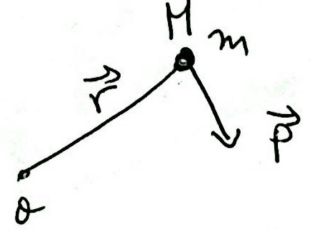
\includegraphics[width=\linewidth]{../pic/2204/conservationmomentangulair.png}
        \end{minipage}
    \end{center}
    \item Conservation de l'énergie mécanique totale
    \item
    \begin{itemize}
        \item Théorème d'énergie cinétique \\
        $\Delta E_c = W$, $W = -\int\vv{F}d\vv{l}$
        \item Forces conservatrices \\
        Si $W_{ACB} = W_{ADB} \implies$ les forces extérieures sont conservatrices
        \item Une condition nécessaire et suffisante pour que $W_{AB}$ soit indépendant du chemin est que $\vv{F}$ dérive d'un potentiel \\
        $\vv{F} = -\vv{grad}(U)$ (U : énergie potentielle)
    \end{itemize}
\end{itemize}
\pagebreak
\section{Contraintes et coordonnées généralisées}
Les contraintes du système introduisent des dépendances entre les coordonnées. Les contraintes sont par exemple des hypothèses de rigidité, limitant son cadre d'évolution, etc.
Exemple :
\begin{itemize}
    \item Pendule simple
    \begin{minipage}{0.49\linewidth}
        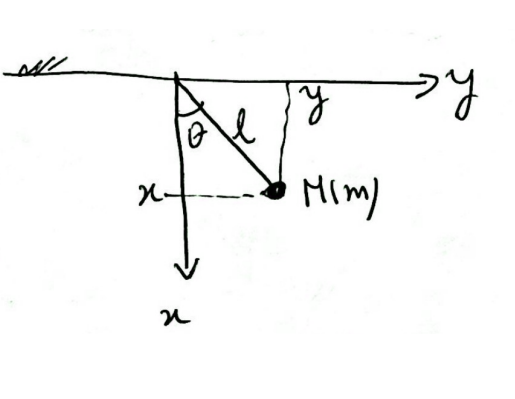
\includegraphics[width=\linewidth]{../pic/2204/pendulesimple.png}
    \end{minipage}
    \begin{minipage}{0.39\linewidth}
        \boxed{x^2 + y^2 = l^2}
    \end{minipage}
    \item Pendule double
    \begin{minipage}{0.49\linewidth}
        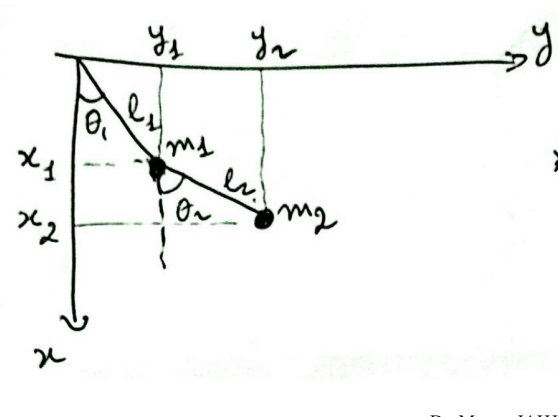
\includegraphics[width=\linewidth]{../pic/2204/penduledouble.png}
    \end{minipage}
    \begin{minipage}{0.39\linewidth}
        \boxed{x_1^2 + y_1^2 = l_1^2} \\
        \boxed{(x_2 - x_1)^2 + (y_2 - y_1)^2 = l_2^2}
    \end{minipage}
\end{itemize}
Système de N particules
\begin{itemize}
    \item Aucune contrainte (indépendantes) $\implies$ 3N coordonnées (3N degrés de liberté)
    \item K contraintes $\implies$ 3N - k coordonnées indépendantes
\end{itemize}
\chapter{Mécanique lagrangienne}
\section{Definition d'un système holonome }
Un système dans lequel on peut déduire l'état d'un système en connaissant seulement les informations sur le changement de positions des composants du système au fil du temps.
\section{Rappel de calcule différentielle}
Soit $f$ une fonction de N variables $f=f(r_1 \ldots , r_N)$
\begin{itemize}
	\item la différentielle totale de $f$ est :
		\[df = \sum^N_{i=1}\frac{\partial f}{\partial r_i}dr_i\]
	\item la derive de $f$ par rapport a l'une de ses variable $(r_j)$ :
	      \[ \frac{df}{dr_j} = \sum^N_{i=1}\frac{\partial f}{\partial r_i}\frac{dr_i}{dr_j} \]
	\item si tout les variable sont independent
	      \[ \frac{df}{dr_j} = \frac{\partial f}{\partial r_j} = \sum^N_{i=1}\frac{\partial f}{\partial r_i}\frac{dr_i}{dr_j} = \sum^N_{i=1}\frac{\partial f}{\partial r_i}\frac{\partial r_i}{\partial r_j} \]
\end{itemize}
\pagebreak
\section{Equation générale de Lagrange }
On considère un system holonome de $N$ particule , $d$ degré du liberté , avec $\vv{F_\alpha}$ est la force appliquée sur la particule $\alpha$
\subsection{L'energie cinétique est :}
$T = \sum^N_{\alpha=1}T_\alpha =\sum^N_{\alpha=1}\frac{1}{2}m_\alpha\vv{\dot{r_\alpha}}^2 $ avec $\begin{cases}
	\vv{r_\alpha} = \vv{r_\alpha}(q_1,q_2,q_3\ldots q_d ,t)\\
	\alpha = 1,2,3 \ldots N\\
	q_i : \text{coordonné généralise} \\
	i=1,2,3\ldots d\\
	\vv{\dot{r}} = \frac{d\vv{r_\alpha} }{dt}
\end{cases}$\\
$T_\alpha = T_\alpha(\underbrace{q_1,q_2\ldots q_d}_{\text{position}} , \underbrace{\dot{q_1},\dot{q_2}\ldots\dot{q_d}}_{\text{vitess}} , \underbrace{t}_{\text{temp}}) $ \\
\subsection{Les forces généralisé associe a $q_i$}
\begin{small}
\begin{itemize}
	\item On a : $dT = \sum^N_{\alpha =1} \frac{\partial T}{\partial \dot{r_\alpha}}d\dot{r_\alpha}$ (differentielle totale de $T$)
	      $\implies \frac{dT}{d\dot{q_i}} = \sum^N_{\alpha =1} \frac{\partial T}{\partial \dot{r_\alpha}}\frac{d\dot{r_\alpha}}{d\dot{q_i}}$ \\
	\item Puisque les variable sont independent alors :\\
	      $ \frac{dT}{d\dot{q_i}}=\frac{\partial T}{\partial\dot{q_i}} = \sum^N_{\alpha =1} \frac{\partial T}{\partial \dot{r_\alpha}}\frac{\partial\dot{r_\alpha}}{\partial\dot{q_i}}$
	      $\implies \frac{\partial T}{\partial \dot{q_i}}=\frac{\partial}{\partial \dot{q_i}}(\sum^N_{\alpha =1} \frac{1}{2}m_\alpha(\vv{\dot{r_\alpha}})^2)= \frac{1}{2}(\sum^N_{\alpha =1} m_\alpha \frac{\partial}{\partial\dot{q_i}}(\vv{\dot{r_\alpha}})^2)$
	      \\ $= \frac{1}{2}\times 2 \sum^N_{\alpha =1} m_\alpha \vv{\dot{r_\alpha}}\frac{\partial \vv{\dot{r_\alpha}}}{\partial\dot{q_i}} \implies$ \boxed{\frac{\partial T}{\partial \dot{q_i}} = \sum^N_{\alpha =1} m_\alpha\vv{\dot{r_\alpha}}\frac{\partial\vv{\dot{r_\alpha}}}{\partial\dot{q_i}}}\\
	\item Chercher $\vv{\dot{r_\alpha}}$ , ona :
	      \begin{itemize}
		      \item $\vv{r_\alpha} = \vv{r_\alpha} (q_1,q_2\ldots q_d , t) $
		      \item $\vv{r_\alpha} = \frac{d((\vv{r_\alpha}))}{dt}$
	      \end{itemize}
	      $d\vv{r_\alpha} = \frac{\partial\vv{r_\alpha}}{\partial q_1}dq_1+\frac{\partial\vv{r_\alpha}}{\partial q_2}dq_2 + \ldots +\frac{\partial\vv{r_\alpha}}{\partial q_d}dq_d+\frac{\partial\vv{r_\alpha}}{\partial t}dt$ \\
	      $\frac{d\vv{r_\alpha}}{dt} =\vv{\dot{r_\alpha}}= \frac{\partial\vv{r_\alpha}}{\partial q_1}\frac{dq_1}{dt}+\frac{\partial\vv{r_\alpha}}{\partial q_2}\frac{dq_2}{dt} + \ldots +\frac{\partial\vv{r_\alpha}}{\partial q_d}\frac{dq_d}{dt}+\frac{\partial\vv{r_\alpha}}{\partial t}$ \\
	      $\frac{d\vv{r_\alpha}}{dt} =\vv{\dot{r_\alpha}}= \frac{\partial\vv{r_\alpha}}{\partial q_1}\frac{\partial q_1}{\partial t}+\frac{\partial\vv{r_\alpha}}{\partial q_2}\frac{\partial q_2}{\partial t} + \ldots +\frac{\partial\vv{r_\alpha}}{\partial q_d}\frac{\partial q_d}{\partial t}+\frac{\partial\vv{r_\alpha}}{\partial t}$ \\
	      \begin{center}
		      \boxed{\vv{\dot{r_\alpha}}= \sum^d_{i =1}\frac{\partial\vv{r_\alpha}}{\partial q_i}\dot{q_i}+\frac{\partial \vv{r_\alpha}}{\partial t}  } avec $\alpha = 1,2\ldots N$
	      \end{center}
	\item démontrer que $\frac{\partial\vv{\dot{r_\alpha}}}{\partial\dot{q_i}} = \frac{\partial\vv{r_\alpha}}{\partial q_i}$ \\
	      $\vv{\dot{r_\alpha}} =\sum^d_{i =1} \frac{\partial\vv{r_\alpha}}{\partial q_i}\dot{q_i} + \frac{\partial r_\alpha}{\partial t} = \frac{\partial \vv{r_\alpha}}{\partial q_1}\dot{q_1} + \ldots+ \frac{\partial \vv{r_\alpha}}{\partial q_i}\dot{q_i} + \ldots + \frac{\partial \vv{r_\alpha}}{\partial q_d}\dot{q_d} +\frac{\partial \vv{r_\alpha}}{\partial t}(q_i,t)$ \\
	      $\frac{\partial}{\partial \dot{q}}\left( \frac{\partial\vv{r}}{\partial t} \right) = 0$ car $\frac{\partial\vv{r}}{\partial t} = \frac{\partial \vv{r}}{\partial t}(q_i,t)$ \\
	      $\frac{\partial \vv{\dot{r_\alpha}}}{\partial\dot{q_i}} = 0 +0 +0 \ldots + \frac{\partial \vv{r_\alpha }}{\partial q_i}\frac{\partial \dot{q_i}}{\partial \dot{q_i}} + \ldots + 0$ \\
	      $=\frac{\partial\vv{r_\alpha}}{\partial q_i} = \frac{\partial\vv{r_\alpha}}{\partial q_i} \implies$\boxed{\frac{\partial\vv{\dot{r_\alpha}}}{\partial\dot{q_i}} = \frac{\partial\vv{r_\alpha}}{\partial q_i}} \\
	\item alors $\frac{\partial T}{\partial \dot{q_i}} =\sum^N_{\alpha =1}m_\alpha \vv{\dot{r_\alpha}}\frac{\partial \vv{\dot{r_\alpha}}}{\partial \dot{q_i}} \implies $ \boxed{\frac{\partial T}{\partial \dot{q_i}} =\sum^N_{\alpha =1}m_\alpha \vv{\dot{r_\alpha}}\frac{\partial \vv{r_\alpha}}{\partial q_i}}\\
	\item Calcule de $\frac{d}{dt}\left( \frac{\partial T}{\partial \dot{q_i}} \right)$ \\
	      \begin{itemize}
		      \item $ \frac{d}{dt}\left( \frac{\partial T}{\partial \dot{q_i}} \right) =\frac{d}{dt}\left( \sum^N_{\alpha = 1}m_\alpha\vv{\dot{r_\alpha}}\frac{\partial \vv{r_\alpha}}{\partial q_i} \right) = \sum^N_{\alpha = 1}m_\alpha \vv{\ddot{r_\alpha}} \frac{\partial \vv{r_\alpha}}{\partial q_i} + \sum^N_{\alpha = 1}m_\alpha\vv{\dot{r_\alpha}}\underbrace{\frac{d}{dt}\left( \frac{\partial \vv{r_\alpha}}{\partial q_i} \right)}$ \\
		      \item Calcule de $\frac{d}{dt}\left( \frac{\partial \vv{r_\alpha}}{\partial q_i} \right)$ \\
		            $d\left( \frac{\partial \vv{r_\alpha}}{\partial q_i} \right) = \sum^d_{i=1}\frac{\partial}{\partial q_i} \left( \frac{\partial \vv{r_\alpha}}{\partial q_i} \right)dq_i + \frac{\partial}{\partial t}\left( \frac{\partial \vv{r_\alpha}}{\partial q_i} \right)dt$\\
		            $\frac{d}{dt}\left( \frac{\partial \vv{r_\alpha}}{\partial q_i} \right) = \sum^d_{i=1}\frac{\partial}{\partial q_i} \left( \frac{\partial \vv{r_\alpha}}{\partial q_i} \right)\dot{q_i} + \frac{\partial}{\partial t}\left( \frac{\partial \vv{r_\alpha}}{\partial q_i} \right) \implies \frac{d}{dt}\left( \frac{\partial \vv{r_\alpha}}{\partial q_i} \right) = \sum^d_{i=1}\frac{\partial}{\partial q_i} \left( \frac{\partial \vv{r_\alpha}}{\partial q_i} \right)\dot{q_i} + \frac{\partial}{\partial q_i}\left( \frac{\partial \vv{r_\alpha}}{\partial t} \right)$\\
		            $\frac{d}{dt}\left( \frac{\partial \vv{r_\alpha}}{\partial q_i} \right) = \frac{\partial}{\partial q_i} \left( \sum^d_{i=1} \frac{\partial\vv{r_\alpha}}{\partial q_i} \dot{q_i} + \frac{\partial}{\partial t}\vv{r_\alpha} \right) = \frac{\partial}{\partial q_i}\vv{\dot{r_\alpha}} = \frac{\partial}{\partial q_i}\frac{d}{dt}(\vv{r_\alpha}) \implies $ \boxed{\frac{d}{dt}\left( \frac{\partial \vv{r_\alpha}}{\partial q_i} \right)= \frac{\partial}{\partial q_i}\vv{\dot{r_\alpha}} } \\
		      \item Verifier que $\sum^N_{\alpha = 1}m_\alpha \vv{\ddot{r_\alpha}} \frac{\partial \vv{r_\alpha}}{\partial q_i} = \frac{\partial T}{\partial q_i} $\\
		            on a $T = \sum^N_{\alpha =1 }m_\alpha\vv{\dot{r_\alpha}}^2 $
		            $\implies \frac{\partial T}{\partial q_i} =  \sum^N_{\alpha =1 }m_\alpha\frac{\partial}{\partial q_i}(\vv{\dot{r_\alpha}})^2 \implies$
		            \boxed{\frac{\partial T}{\partial q_i}= \sum^N_{\alpha =1 }m_\alpha\vv{\dot{r_\alpha}}\frac{\partial \vv{\dot{r_\alpha}}}{\partial q_i}}
	      \end{itemize}
	      alors \begin{center}
		      \boxed{\frac{d}{dt}\left( \frac{\partial T}{\partial \dot{q_i}} \right) =\frac{\partial T}{\partial q_i} + \sum^N_{\alpha = 1}m_\alpha\vv{\dot{r_\alpha}}\frac{\partial}{\partial q_i}\vv{\dot{r_\alpha}} }
	      \end{center}
	\item on utilise la loi de Newton : $ \vv{F_\alpha} = m_\alpha\vv{\ddot{r_\alpha}} \implies  \frac{d}{dt}\left( \frac{\partial T}{\partial \dot{q_i}} \right) =\frac{\partial T}{\partial q_i} + \sum^N_{\alpha = 1}\vv{F_\alpha}\frac{\partial\vv{\dot{r_\alpha}}}{\partial q_i}$  \\
	      avec $\sum^N_{\alpha = 1}\vv{F_\alpha}\frac{\partial\vv{\dot{r_\alpha}}}{\partial q_i} = Q_i$
	      \begin{center}
			\boxed{Q_i = \frac{d}{dt}\left( \frac{\partial T}{\partial \dot{q_i}} \right) - \frac{\partial T}{\partial q_i}}
		\end{center}
\end{itemize}
\end{small}

\pagebreak
\section{Formalisme de Lagrange : cas d un system conservatif}
\begin{itemize}
	\item Si les forces $\vv{F_\alpha}$ sont conservatif , on suppose que toutes les forces agissant sur ce system dérivent d'une mem énergie potentielle $U$ \\
	      avex $U$ depend de position $U = U(\vv{r_1}, \vv{r_2}\ldots , \vv{r_N})$ et $\vv{F_\alpha}=-\vv{grad}U$ \\
	      Donc , on a \boxed{\sum^N_{\alpha =1 }\vv{F_\alpha}d\vv{r_\alpha}=-dU}
	\item On a l equation de Lagrange $\frac{d}{dt}\left( \frac{\partial T}{\partial \dot{q_i}} \right) - \frac{\partial T}{\partial q_i} = \sum^N_{\alpha = 1}\vv{F_\alpha}\frac{\partial\vv{\dot{r_\alpha}}}{\partial q_i} = Q_i$ \\
	      avec $Q_i =\sum^N_{\alpha = 1}\vv{F_\alpha}\frac{\partial\vv{\dot{r_\alpha}}}{\partial q_i} = \frac{-dU}{dq_i}\implies $ \boxed{Q_i =\frac{-\partial U}{\partial q_i}}(si les forces sont conservatives)
	\item L'equation devien $\frac{d}{dt}\left( \frac{\partial T}{\partial \dot{q_i}} \right) - \frac{\partial T}{\partial q_i} = \frac{-\partial U}{\partial q_i} \implies \frac{d}{dt}\left( \frac{\partial T}{\partial \dot{q_i}} \right) = \frac{-\partial}{\partial q_i}(T-U) =0$
	\item U depend seulment du position alors $\frac{\partial T}{\partial \dot{q_i}} = \frac{\partial}{\partial \dot{q_i}}(T-U)$ \\
	      l equation devien $\frac{d}{dt}\left( \frac{\partial}{\partial \dot{q_i}}(T-U) \right) - \frac{\partial}{\partial q_i} (T-U) =0$
	\item On introduis la fonction de Lagrange (Lagrangien) \\
	      \begin{center}
		      \boxed{L(qi,\dot{q_i},t) = T- U } \\
		      $T$ depend de vites $\dot{q_i}$ et $U$ depend de position $q_i$
	      \end{center}
	\item L equation devient \\
	      \begin{center}
		      Equation Euler-Lagrange : \boxed{\frac{d}{dt}\left( \frac{\partial L}{\partial \dot{q_i}} \right) - \frac{\partial L}{\partial q_i} =0}
	      \end{center}
\end{itemize}

\section{Les lois de conservation }
\begin{itemize}
	\item Invariance par temps : ENERGIE
	      \\ pour le démontre :$ \frac{\partial L}{\partial t} = 0 \implies   $ t est un variable cyclique \\
	      on applique Beltrami : $ L - \frac{\dot{q}\partial L}{\partial \dot{q}} = cte $ ... jusqu' arrive a $  U + T = cte$
	\item Invariance par translation  : QUANTITÉ DE MOUVEMENT 
	      \\ pour le démontre : si $ q_\alpha $ est un variable cyclique $ \implies \frac{\partial L}{\partial \alpha} = 0 \implies   $ la quantité du mouvement $ p_\alpha = cte $
	\item Invariance par rotation : MOMENT CINÉTIQUE  \\
	      pour le démontre : Si $ \theta  $ une coordonné généralisé angle est cyclique $ \implies \vv{\mathfrak{L}} = cte  $ \\
	      note que le moment cinétique est : $ \vv{\mathfrak{L}} = \vv{r} \wedge \vv{p} $
\end{itemize}
\section{Beltrami \& Moindre d'action}
\subsection{Moindre d'action}
$ \delta S = \int \delta L dt =0 \Longleftrightarrow \frac{d}{dt}(\frac{\partial L}{\partial \dot{q_i}}) - \frac{\partial L}{\partial q_i} =0  $
\subsubsection{Lagrange a partir du moindre action}
\begin{itemize}
	\item Soit $ S $ est l 'action du système \\
	      $ S = \int_{t_1}^{t_2}L(q_i,\dot{q_i},t)dt$
	\item Le principe de moindre d'action stipule que le système évolue de la position $ q_1 $ a la position $ q_2 $  de telle façon que $ S $ est la plus petite valeur possible $ \implies \delta S = 0 $ \\
	      $ \delta S = \int_{t_1}^{t_2} \delta L dt = \int_{t_1}^{t_2} \left[ L(q + \delta q , \dot{q} + \delta \dot{q} , t) - L ( q , \dot{q} , t) \right] dt =0  $
	\item En se limitant dans le développement de Taylor de l'integrant suivant les puissance de $ \delta q $ et $ \delta \dot{q} $ aux termes de premier ordre , on obtient : \\
	      $ \delta S = \int_{t_1}^{t_2} (\frac{\partial L}{\partial q}\delta q + \frac{\partial L}{\partial \dot{q}}\delta \dot{q})dt = 0 $
	\item  On a : $ \delta \dot{q} = \frac{d}{dt}\delta q  $ \\
	      $ \implies \delta S = \frac{\partial L}{\partial \dot{q}}\delta q ]^{t_2}_{t_1} + \int_{t_1}^{t_2} ( \frac{\partial L}{\partial q} - \frac{d}{dt}\frac{\partial L}{\partial \dot{q}})\delta q dt =0$
	\item $ \frac{\partial L}{\partial \dot{q}}\delta q ]^{t_2}_{t_1}  =0 $
	\item L'integral doit être nulle pour tout $ \delta q $ , ceci n'est possible que si l'integrant est identiquement null \\
	      \begin{center}
		      $ \implies  $ \boxed{\frac{d}{dt}(\frac{\partial L}{\partial \dot{q}}) - \frac{\partial L}{\partial q} = 0}
	      \end{center}
\end{itemize}
\subsection{Beltrami}
Si t est une variable cyclique alors : \\
$ L - \dot{q_i}\frac{\partial L}{\partial \dot{q_i}} = cte \Longleftrightarrow \frac{d}{dt}(\frac{\partial L}{\partial \dot{q_i}}) - \frac{\partial L}{\partial q_i} =0 $
\subsubsection{Lagrange a partir de Beltrami}
Identité de Beltrami : $ L - \dot{q} \frac{\partial L}{\partial \dot{q}} = cte  $ \\
$ \left(L - \dot{q} \frac{\partial L}{\partial \dot{q}} = cte \right)\times \frac{d}{dt} $ avec $ \begin{cases} dL = \frac{\partial L}{\partial q}dq + \frac{\partial L}{\partial \dot{q}}d\dot{q}\\ \frac{dL}{dt}=\frac{\partial L}{\partial q}\dot{q} + \frac{\partial L}{\partial \dot{q}}\ddot{q}                \end{cases} $\\
$ \frac{\partial L}{\partial q}\dot{q} + \frac{\partial L}{\partial \dot{q}}\ddot{q} - \frac{\partial L}{\partial \dot{q}}\ddot{q} - \dot{q}\frac{d}{dt}(\frac{\partial L}{\partial \dot{q}}) = 0 $\\
$ \dot{q}\left[ \frac{\partial L}{\partial q} - \frac{d}{dt}(\frac{\partial L}{\partial \dot{q}}) \right] = 0 \\
	\implies$ \boxed{ \frac{\partial L}{\partial q} - \frac{d}{dt}(\frac{\partial L}{\partial \dot{q}}) = 0}

\subsection{Trajectoire du lumière }
\begin{small}
$ T = \int dt = \int \frac{dl}{v} = \int \frac{\sqrt{1+y'^2}}{c}\times n dx $ avec $ n :\text{ indice de refraction } n(x,y) $ \\
( On peut pas utilise Beltrami car x n'est pas un variable cyclique ( n depend de x))\\
$ \delta T = 0 \implies \int \delta \left( \frac{\sqrt{1+y'^2}}{c} \times n \right)dx = 0 $ \\
$ f(x,y,y') = \frac{\sqrt{1+y'^2}}{c}\times n \implies \int\delta f dx =0 \\
	\implies \frac{d}{dx}(\frac{\partial f}{\partial y'}) - \frac{\partial f}{\partial y}  = 0 \text{ ( Euler-Lagrange )}\\
$
\begin{itemize}
	\item   $ \frac{\partial f}{\partial y'} = \frac{1}{c}n\frac{1}{2}\frac{2y'}{(1+y'^2)^{\frac{1}{2}}} = \frac{ny'}{c(1+y'^2)^{\frac{1}{2}}} $
	\item $\frac{d}{dx}(\frac{\partial f}{\partial y'}) = \frac{d}{dx}n(\frac{y'}{c(1+y'^2)^{\frac{1}{2}}}) + \frac{n}{c}\frac{d}{dx}(\frac{y'}{(1+y^2)^{\frac{1}{2}}}) \\
		      =\left( \frac{\partial n}{\partial y}\frac{dy}{dx} + \frac{\partial n}{\partial x}\frac{dx}{dx} \right)(\frac{y'}{c(1+y'^2)^{\frac{1}{2}}})+ \frac{n}{c}\left( \frac{y''}{\sqrt{1+y'^2}}+y'(\frac{-1}{2})2y'y''(1+y'^2)^{\frac{-3}{2}} \right)\\
		      = \left( \frac{\partial n}{\partial y}y' +\frac{\partial n}{\partial x} \right)(\frac{y'}{c\sqrt{1+y'^2}}) + \frac{ny''}{c\sqrt{1+y'^2}}-\frac{n}{c}\frac{y'^2y''}{(1+y'^2)^{\frac{3}{2}}}
	      $
\end{itemize}
$ \implies \left( \frac{d}{dx}(\frac{\partial f}{\partial y'}) - \frac{\partial f}{\partial y} = 0 \right) \times(\sqrt{1+y'^2}\times c)  $\\
$ \implies $ \boxed{ny'' - \frac{\partial n}{\partial y} + y' \frac{\partial n}{\partial x} - \frac{n y'^2 y''}{\sqrt{1+y'^2}} = 0} \\
Pour n = cte $ \implies ny'' - \frac{ny'^2y''}{(1+y'^2)} = 0 \implies y' =a \implies y = ax+b $
\end{small}
\subsection{minimize la distance entre deux points }
\begin{small}
$ T = \int dl \implies T = \int \sqrt{1+y'^2}dx $ ($  dl^2 = dx^2 + dy^2 $ )\\
$ \delta T = \int \delta (\sqrt{1+y'^2})dx = 0 $ , Soit $ f(y') = \sqrt{1+y'^2} \implies \int\delta f dx =0 $ \\
$ \implies f -y' \frac{df}{\partial y'} = cte $ (Beltrami) \\
$ \sqrt{1+y'^2} - y' \frac{\partial\sqrt{1 + y'^2}}{\partial y'} = cte  $\\
$ \sqrt{1 + y'^2} -2y'^2\frac{1}{2}\frac{1}{\sqrt{1+y'^2}} = cte  $\\
$ \frac{1}{\sqrt{1+y'^2}} = cte \implies y' =cte \implies  $ \boxed{y = ax+b}
\end{small}
\subsection{Minimize le temp entre deux point avec un potentiel}
\begin{small}
$ T = \int dt = \int\frac{dl}{v} = \int\frac{\sqrt{1+y'^2}}{v}dx $\\
D'apres la conservation de l'énergie : $ \frac{1}{2}mv_i^2 + mgy_i = \frac{1}{2}mv^2 + mgy_m \implies 0 = mgy_m +\frac{1}{2}mv^2  $ avec $ y_m = - y $ \\
$ \implies  $ \boxed{v = \sqrt{2gy}}\\
$ T = \int \frac{\sqrt{1+y'^2}}{\sqrt{2gy}}dx $ \\
$ \delta T = \int \delta \frac{\sqrt{1+y'^2}}{\sqrt{2gy}}dx  = 0 $\\
$ \implies \frac{\sqrt{1+y'^2}}{\sqrt{2gy}} - y' \frac{\partial \frac{\sqrt{1+y'^2}}{\sqrt{2gy}}}{\partial y'} = cte $ (Beltrami) \\
$ \implies \frac{1}{\sqrt{2gy}}(\frac{1}{\sqrt{1+y'^2}}) =cte  $\\
$ \implies $ \boxed{1+y'^2 = \frac{cte}{y}}
\end{small}
\chapter{Mécanique des fluides }
\section{Hydrostatique}
L'hydrostatique est un branche de la physique qui traite des caractéristiques des fluides au repos.
\subsection{La Pression}
La pression est une mesure de la force exercée sur une unité de surface. 
\begin{itemize}
	\item La Pression : $ P =\frac{\text{Force}}{Surface} =\frac{F}{A} $ , unite : Pascal ($Pa$)  \\
	\item La Pression a un profond h dans un fluid est : $ P = \rho g h $ avec $ \rho $ est la mass volumique de fluid \\
	\item La Pression atmosphérique est $ P_0 = 1 atm =1.013\times 10^5 Pa $
\end{itemize}
\subsection{Loi d’Archimède}
Tout corps plongé dans un liquide subit une poussée verticale vers le haut égale au poids du volume de liquide déplacé \\
$ B = \rho_\text{fluid}gV_\text{volume de l'objet} $
\section{Hydrodynamique}
L'hydrodynamique est un branche de la physique qui a pour objet l'étude des liquides en mouvement.
\section{Definitions}
\begin{minipage}{0.5\linewidth}
	\begin{itemize}
		\item Écoulement laminaire : \\
		      Dans un écoulement laminaire, deux particules de fluide voisines à un instant donné restent voisines aux instants suivants.
		\item Écoulement turbulent : \\
		      l'écoulement turbulent est le mouvement irrégulier des particules du fluide. L'écoulement est chaotique, présentant des tourbillons et une forte instabilité.
	\end{itemize}
\end{minipage}
\begin{minipage}{0.5\linewidth}
	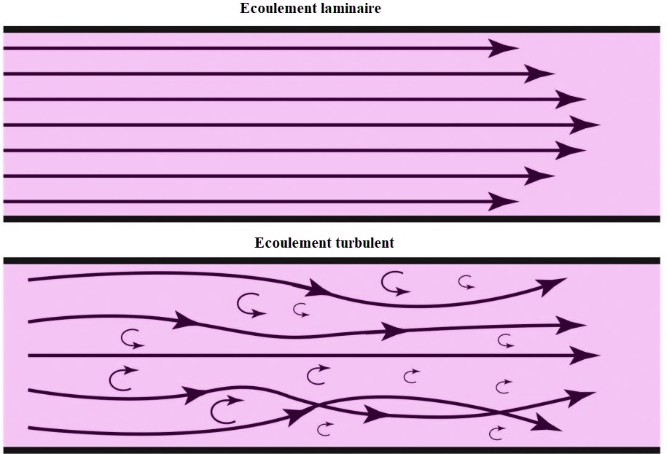
\includegraphics[width=\linewidth]{../pic/1103/1.png}
\end{minipage}
\begin{itemize}
	\item Viscosité : c'est la degré de frottement interne d'un fluide.
\end{itemize}
\section{Écoulement ideal}
Pour l’écoulement sera ideal :
\begin{itemize}
	\item le fluid est non visqueux (fortement interne negligible)
	\item le fluid est stationer ( vites a chaque point reste constant )
	\item le fluid incompressible ($ \rho $ rest constant  )
	\item le fluid irrotationnel ( fluide ne possède pas un moment angulaire )
\end{itemize}
\subsection{Debit}
\begin{itemize}
	\item Debit volumique : \\
	$ D_v = \frac{\text{Volume}}{\text{Temp}} = \frac{\text{Surface} \times \text{Longuer}}{\text{Temp}} = \text{Vitess du fluid} \times \text{Surface} = V\times A  $
	\item Debit massique :\\
	 $ D_m = \frac{\text{mass}}{\text{Temp}} = \frac{\text{ mass volumique} \times \text{Volume}}{\text{Temp}} = \frac{\text{ mass volumique} \times \text{Surface} \times \text{Longuer}}{\text{Temp}} = V\times \rho \times A $
	\item
	      \begin{minipage}{0.5\linewidth}
		      Equation de Continuité de Debit :\\
			   $A_1V_1=A_2V_2 $
	      \end{minipage}
	      \begin{minipage}{0.5\linewidth}
		      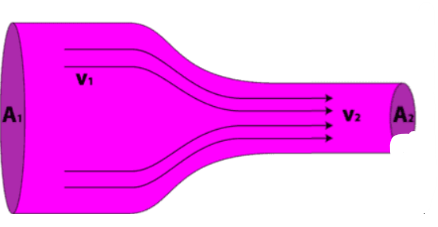
\includegraphics[width=\linewidth]{../pic/1103/2.png}
	      \end{minipage}
\end{itemize}
\section{Equation de Bernoulli}
Dans le flux d'un fluide homogène et incompressible soumis uniquement aux forces de pression et de pesanteur, une accélération se produit simultanément avec la diminution de la pression. \\
\begin{minipage}{0.5\linewidth}
	$ P_1 + \frac{1}{2}\rho V_1^2 + \rho gh_1 = P_2 + \frac{1}{2}\rho V_2^2+\rho g y_2 $
\end{minipage}
\begin{minipage}{0.5\linewidth}
	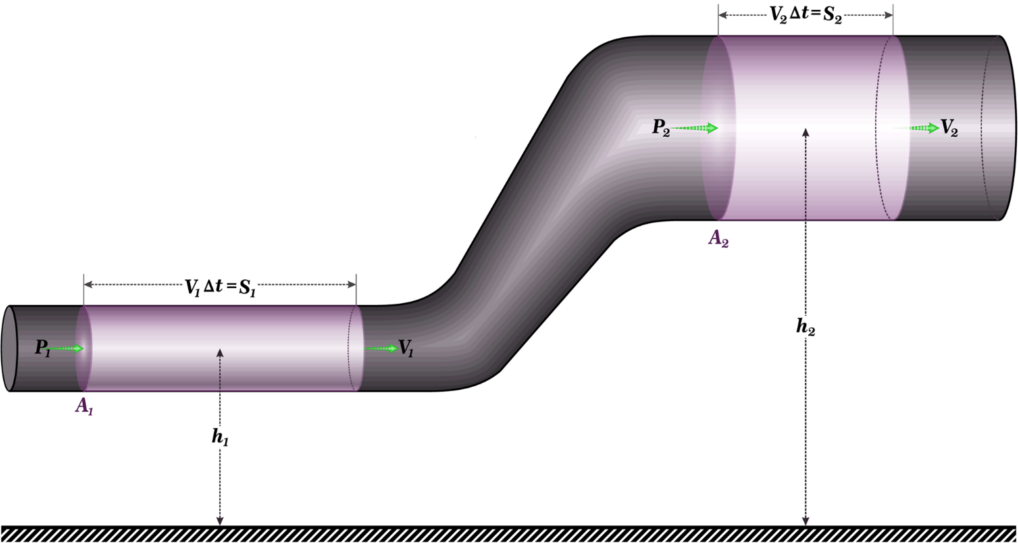
\includegraphics[width=\linewidth]{../pic/1103/3.png}
\end{minipage}
\section{Tension du surface}
\begin{itemize}
	\item La force \underline{cohesives} est la force d'attraction entre les molecule de meme fluid .
	\item La force \underline{adhesive} est la force d'attraction entre les molecule de fluid et une surface en contact avec ce fluid .
\end{itemize}
\begin{minipage}{0.5\linewidth}
	\begin{itemize}
		\item Lorsque la force cohesive du fluid est plus grand que cell adhesives avec la paroi , le fluid se concave ver le bas pour reduire le contact avec le paroi
		\item Lorsque la force adhesive avec la paroi est plus grand que cell cohesive du fluid , le fluid est plus attire par la paroi que par lui meme , le fluid se concave ver le haut .
	\end{itemize}
\end{minipage}
\begin{minipage}{0.5\linewidth}
	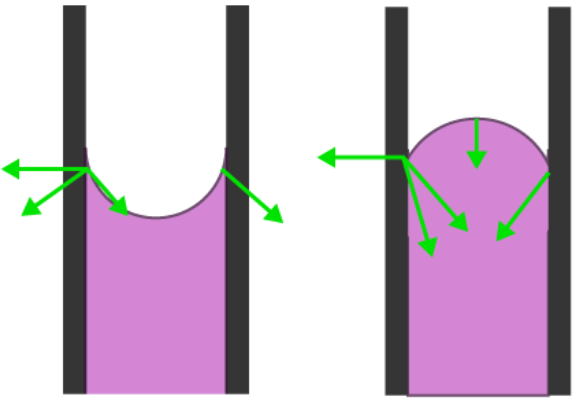
\includegraphics[width=\linewidth]{../pic/1103/4.png}
\end{minipage}
\pagebreak
\subsection{Capillarité}
est le processus d'écoulement d'un liquide dans un espace étroit sans aide , ou même en opposition à des forces extérieures comme la gravité. \\
\begin{minipage}{0.7\linewidth}
	L'hauteur de colone du liquide est : $ h =\frac{2\gamma \cos(\theta)}{\rho g r} $ \\
	avec : \begin{itemize}
		\item $ \gamma :$ est la tension du surface entre le fluid et l'air .
		\item $ \theta : $ est l'angle de contact .
		\item $ \rho : $ est la densite de fluid
		\item $ r : $ est le rayon du tube .
	\end{itemize}
\end{minipage}
\begin{minipage}{0.3\linewidth}
	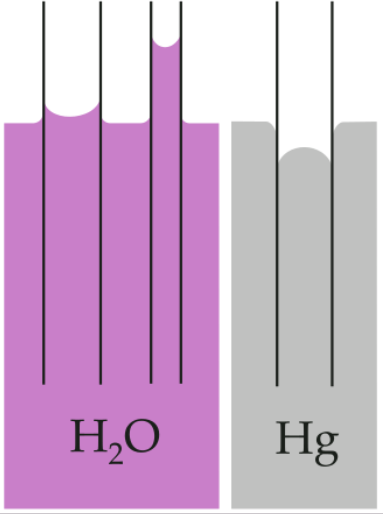
\includegraphics[width=\linewidth]{../pic/1103/5.png}
\end{minipage}
\section{Coefficient de viscosité}
La viscosité dynamique est une grandeur physique qui caractérise la résistance à l'écoulement laminaire d'un fluide.\\
\begin{minipage}{0.7\linewidth}
	La magnitude de force F agissant sur le plaque supérieur varie proportionnel avec la vitesse (u) et la surface (A) de chaque plaque et inversement proportionnel a la distance de separation entre les plaque y \\
	\[F = \frac{\mu\times A \times V=u}{y}\] 
	avec $ \mu : $ est le coefficient de viscosité
\end{minipage}
\begin{minipage}{0.3\linewidth}
	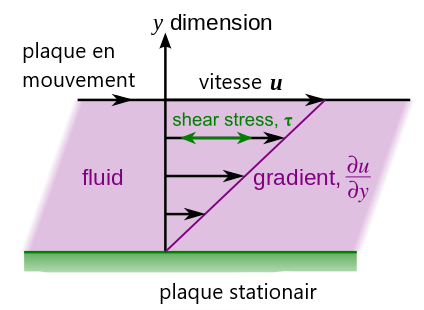
\includegraphics[width=\linewidth]{../pic/1103/6.png}
\end{minipage}
\section{Loi de Poiseuille}
Le loi de Poiseuille décrit l’écoulement laminaire d'un liquide visqueux dans une conduite cylindrique
\begin{minipage}{0.5\linewidth}
	Debit Volumique : $ D_v = \frac{\Delta V}{\Delta t} = \frac{\pi R^4 (P_e - P_s)}{8\mu L} $
\end{minipage}
\begin{minipage}{0.5\linewidth}
	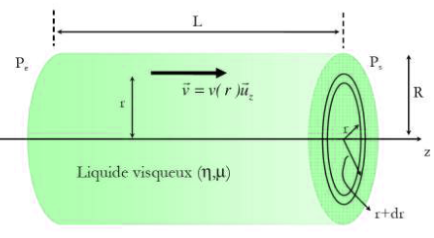
\includegraphics[width=\linewidth]{../pic/1103/7.png}
\end{minipage}
\section{Nombre de Reynolds}
Le nombre de Reynolds représente le rapport entre les forces d'inertie et les forces visqueuses. \\
\begin{center}
	$ R = \frac{V L \rho}{\mu}   $\qquad  $ \begin{cases}
			R < 2000 \implies \text{ecoulement laminaire}       \\
			2000 < R < 3000 \implies \text{ecoulement instable} \\
			3000 < R \implies \text{ecoulement turbulent}
		\end{cases} $
\end{center}
avec :\begin{itemize}
	\item V : vitesse du fluide
	\item $ L$ : Dimension caractéristique( longueur de la plaque , diamètre intérieur du tube ...)
	\item $ \mu $ : Coefficient de viscosité .
	\item $ \rho : $ masse volumique
\end{itemize}
\section{Diffusion}
Le Diffusion est le déplacement des molecule de region plus concentré a une region moins concentre . \\
Debit de diffusion :  $\Phi = DA(\frac{C_2- C_1}{L})  $ avec : \begin{itemize}
	\item A : surface
	\item D : Coefficient de diffusion
	\item C : concentration
	\item L : Distance entre $ C_1 $ et $ C_2 $
\end{itemize}
\section{Loi de Stokes}
La force de viscosité sur une petite sphère se déplaçant à travers un fluide visqueux est donnée par \\
$ \boxed{F = 6\pi \mu rv }$ avec \begin{itemize}
	\item $r$ : le rayon du sphere
	\item $ v: $ : le vitesse de sphere
\end{itemize}




\end{document}